\paragraph{Применение АР-метода для детектирования сигнала с расширенным спектром}

Рассмотрим применение данного подхода для детектирования одного сигнала ШПС на фоне аддитивного белого шума.
Схема алгоритма представлена на рисунке \ref{pic:ar_cdma1_scheme1}.

\begin{figure}[H]
	\center\scalebox{0.9}{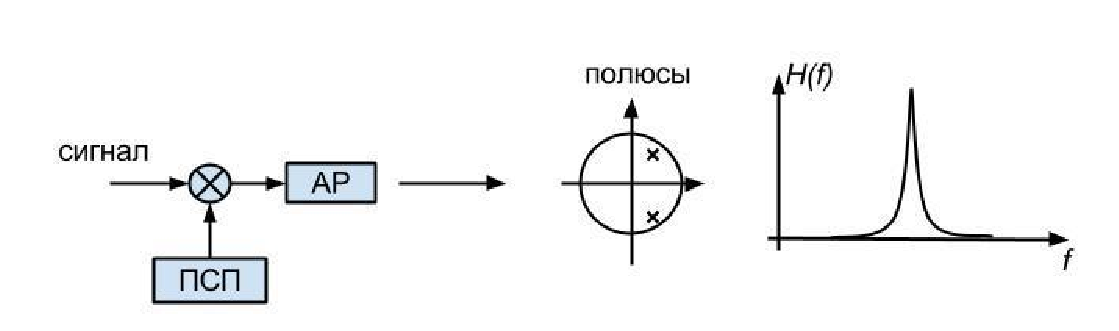
\includegraphics[width=1\linewidth]{lpc_for_1_sat_scheme.eps}}
	\caption{Детектирование сигнала АР-методом при известной фазе ПСП.}
	\label{pic:ar_cdma1_scheme1}
\end{figure}

Для восстановления гармонического сигнала из ШПС входная последовательность умножается на локально сформированную ПСП.
Далее запускается алгоритм на основе АР-модели. В реальных условиях приемник не имеет информации о фазе ПСП поэтому для детектирования
сигнала необходимо перебрать все возможные смещения расширяющего кода. Для ускорения вычислений предлагается использование алгоритма быстрого преобразования Фурье (БПФ).
Схема вычислений представлена на рисунке \ref{pic:ar_cdma1_scheme2}.

\begin{figure}[H]
	\center\scalebox{0.9}{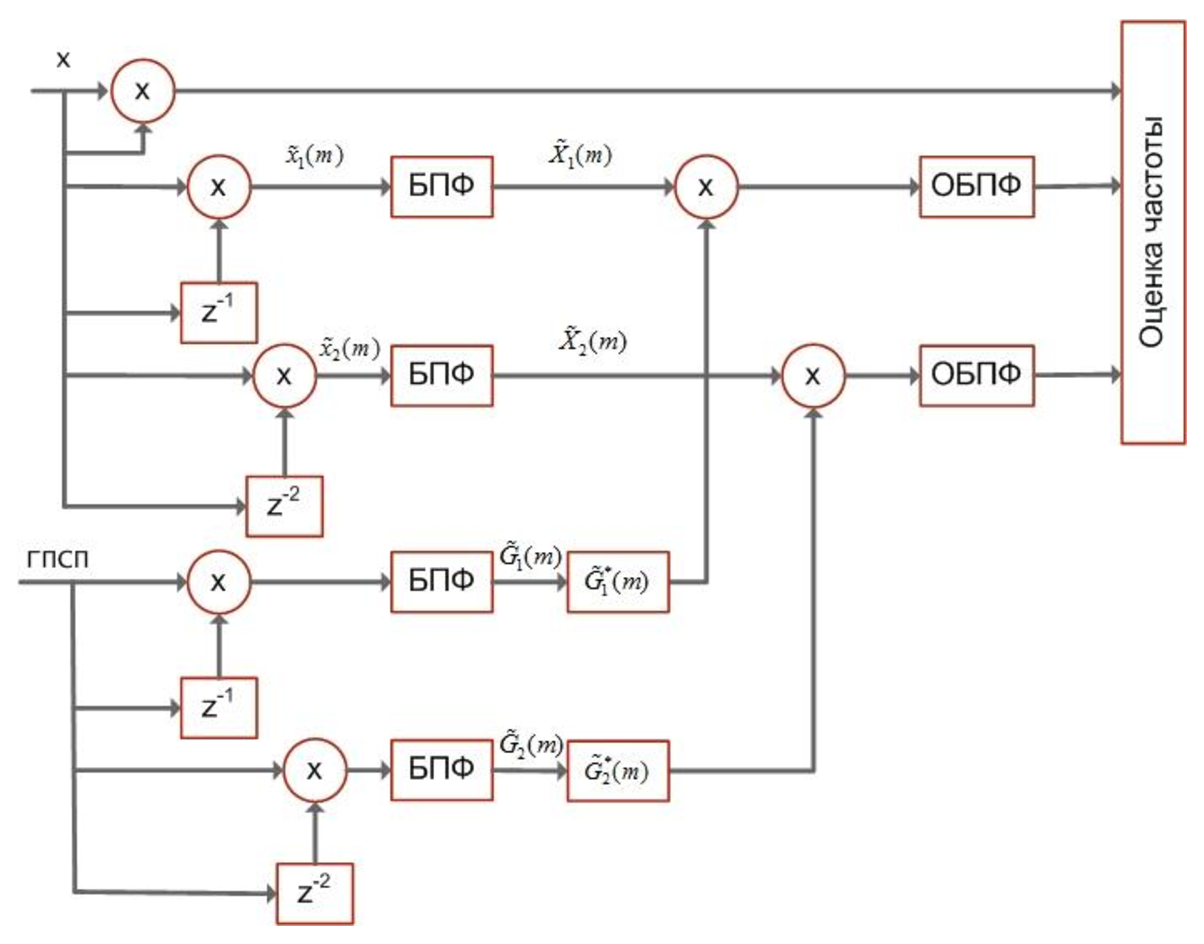
\includegraphics[width=1\linewidth]{lpc_fft.eps}}
	\caption{Общая схема применения АР модели для детектирования ШПС сигнала.}
	\label{pic:ar_cdma1_scheme2}
\end{figure}

Оценка ${\hat{r}_{xx}(0)}$ не зависит от выбранной фазы ПСП, поэтому она вычисляется один
раз для всех смещений кода. Далее формируется массив произведений входного сигнала на
свою задержанную копию ${\tilde{x}_1(n)=x(n)x(n-1)}$. Полученная последовательность  
${\tilde{x}_1(n)}$ поступает на вход алгоритма БПФ, в результате получаем массив ${\tilde{X}_1(n)}$
содержащий частотные отсчеты. Аналогично формируется массив  ${\tilde{X}_2(n)}$ для
задержки входного сигнала равной двум. Таким же способом обрабатываются локально
сгенерированные ПСП и формируются два массива ${\tilde{C}_1(n)}$ и ${\tilde{C}_2(n)}$.
Далее массивы ${\tilde{X}_1(n)}$ и ${\tilde{X}_1(n)}$ поэлементно перемножаются
на комплексно сопряженные массивы ${\tilde{C}_1^*(n)}$ и ${\tilde{C}_2^*(n)}$.
Результаты этих перемножений поступают на вход алгоритма обратного
БПФ. Полученные после ОБПФ два массива содержат оценки автокорреляционной функции для ${N}$ 
смещений кода, где  ${N}$ - размер данных на входе алгоритма БПФ.

Таким образом, предлагаемый алгоритм состоит из следующих шагов:

\begin{itemize}
\item[Шаг 1.] Вычисляются оценки  АКФ в трех первых точках (для аргументов АКФ=0,1,2)
	с использованием алгоритма БПФ для всех возможных смещений ПСП. 
\item[Шаг 2.] Для каждого смещения ПСП: 
	Определяются коэффициенты АР-модели ${\hat{a_1}, \hat{a_2}}$, 
	по формуле \ref{eq:ar_coef_matrix}.
	Вычисляется резонансная частота ${\omega_0}$
	и определяется квадрат модуля частотного отклика АР-модели для этой частоты. 
\item[Шаг 3.] Выбирается смещение ПСП для которого значение квадрата модуля частотного отклика было максимальным. Полученное значение сравнивается с заранее выбранным порогом детектора. 
	\subitem{\bf{Если}}  значение оказалось больше порогового {\bf{то}} 
		принимается решение о наличии сигнала, а в качестве оценки
		частоты принимается значение ${\omega_0}$ соответствующее выбранному смещению ПСП. 
	\subitem{\bf{Иначе}} 
		Принимается решение об отсутствии гармонического сигнала.
\end{itemize}

Разработанный алгоритм позволяет производить оценку частоты гармонического сигнала без использования прямого перебора как это делается в большинстве современных алгоритмов.
Например, алгоритм Delay and Multiply Approach (DMA) предложенный в \cite{tsui,lin_dma} позволяет производить поиск только по смещению ПСП,
но он не дает возможности прямой оценки частоты. Для оценки частоты и принятия решения о наличии сигнала в алгоритме DMA необходимо использовать стандартный коррелятор.
Предложенный алгоритм допускает сокращение количества операций умножения при переборе значений фазы ПСП за счет использования алгоритма БПФ.

\begin{figure}[H]
	\center\scalebox{1}{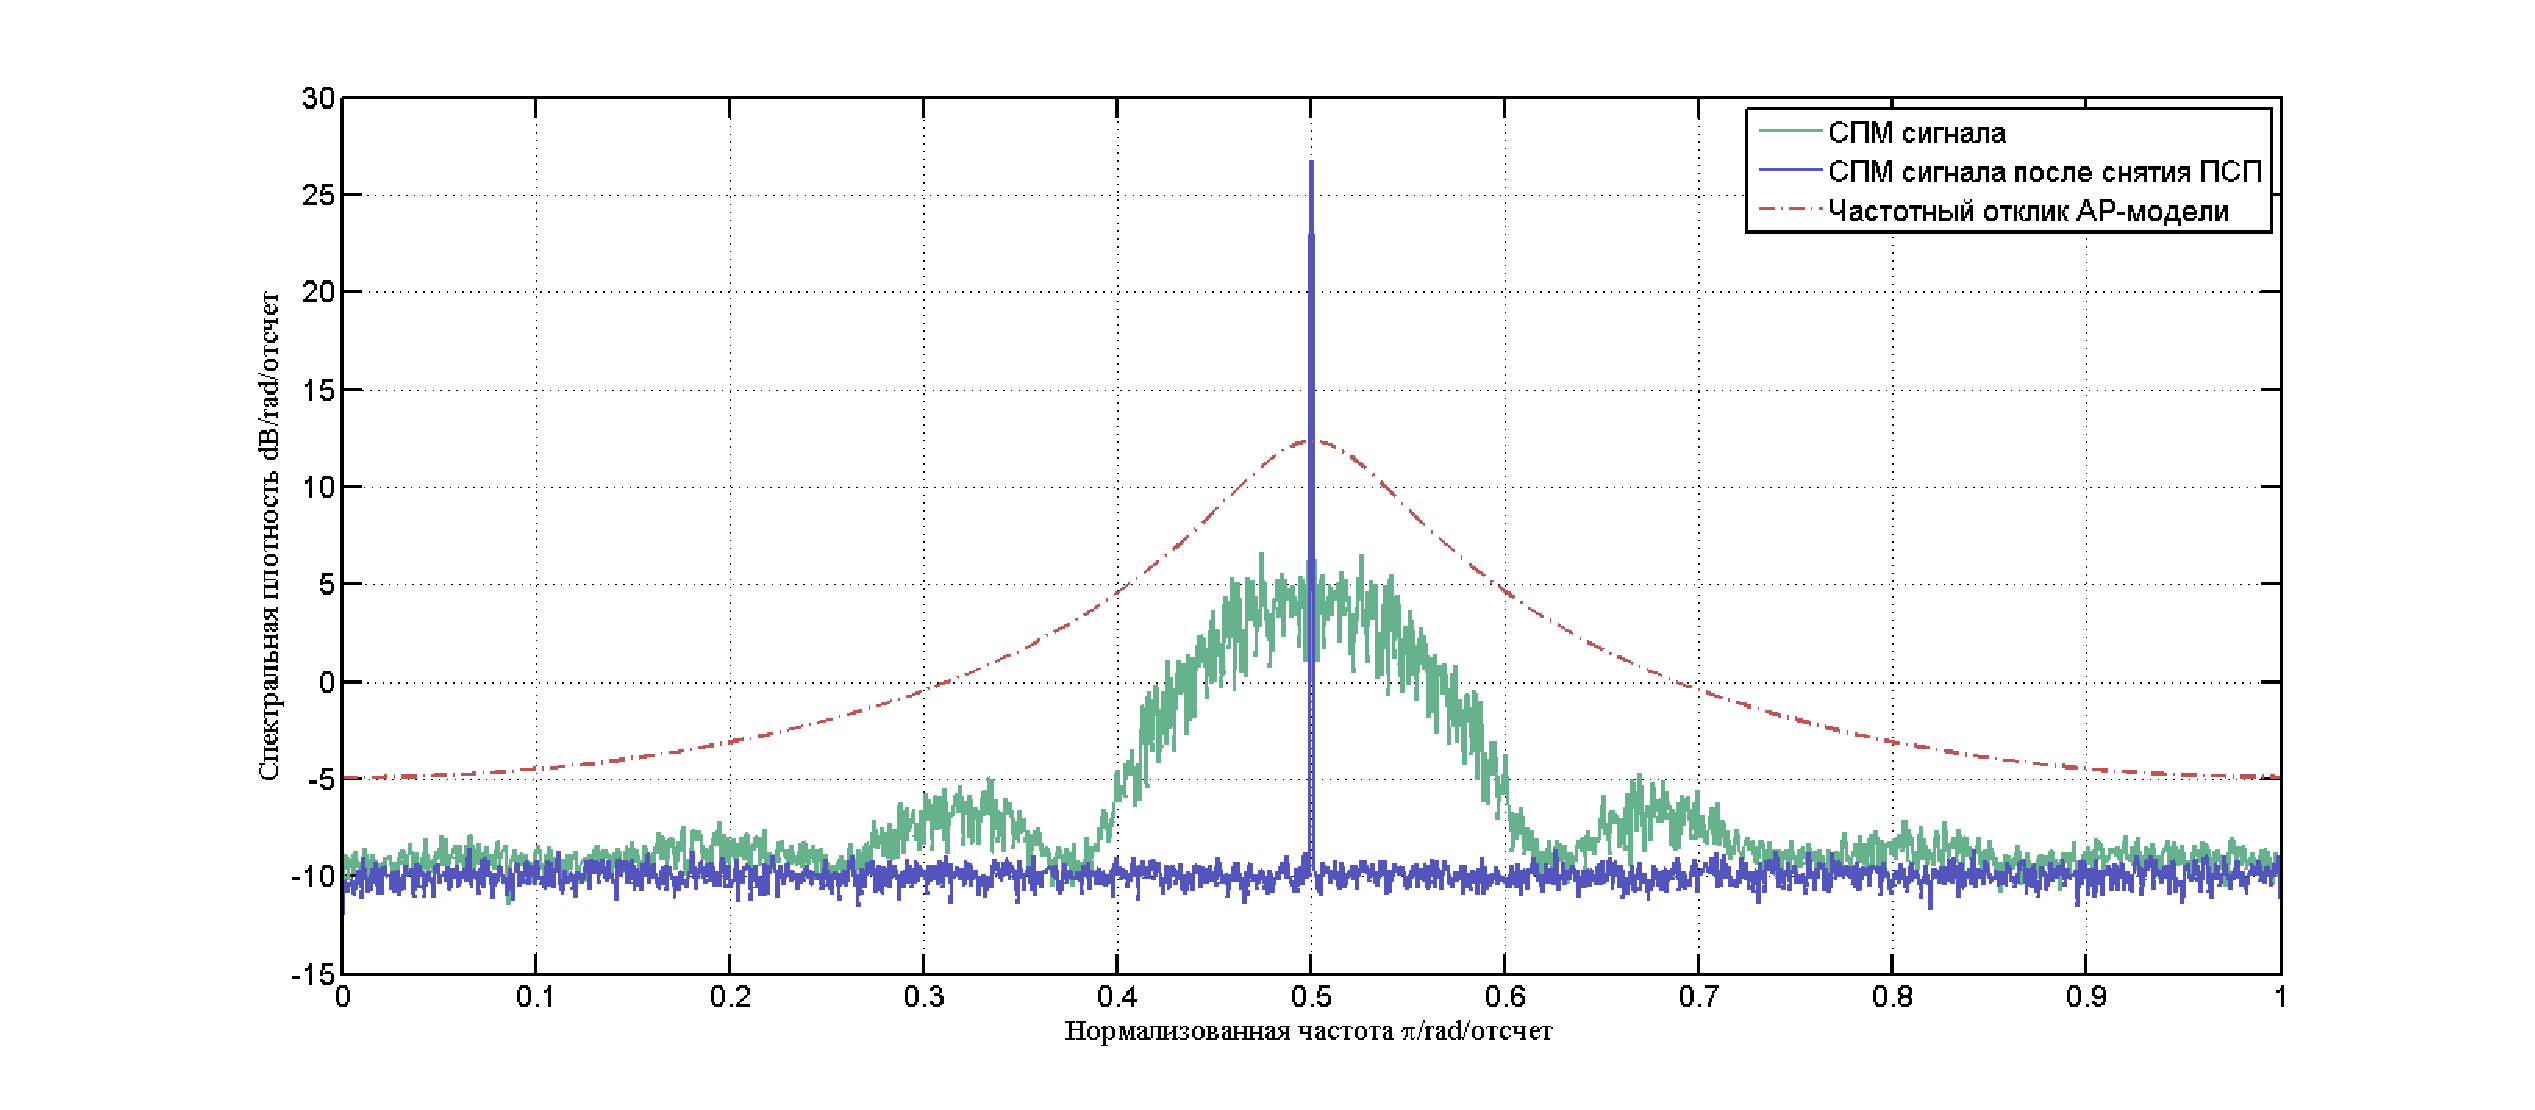
\includegraphics[width=1\linewidth]{lpc_1sat.eps}}
	\caption{Оценка СПМ сигнала модулированного ПСП}
	\label{pic:ar_cdma1_freq_est1}
\end{figure}

Основным недостатком предложенного алгоритма является сильная чувствительность по отношению к интерференционным помехам: наличие «окрашенного» шума приводит к
значительному смещению получаемых оценок частоты и мощности гармонического сигнала - рисунок \ref{pic:ar_cdma1_freq_est2}.

\begin{figure}[H]
	\center\scalebox{1}{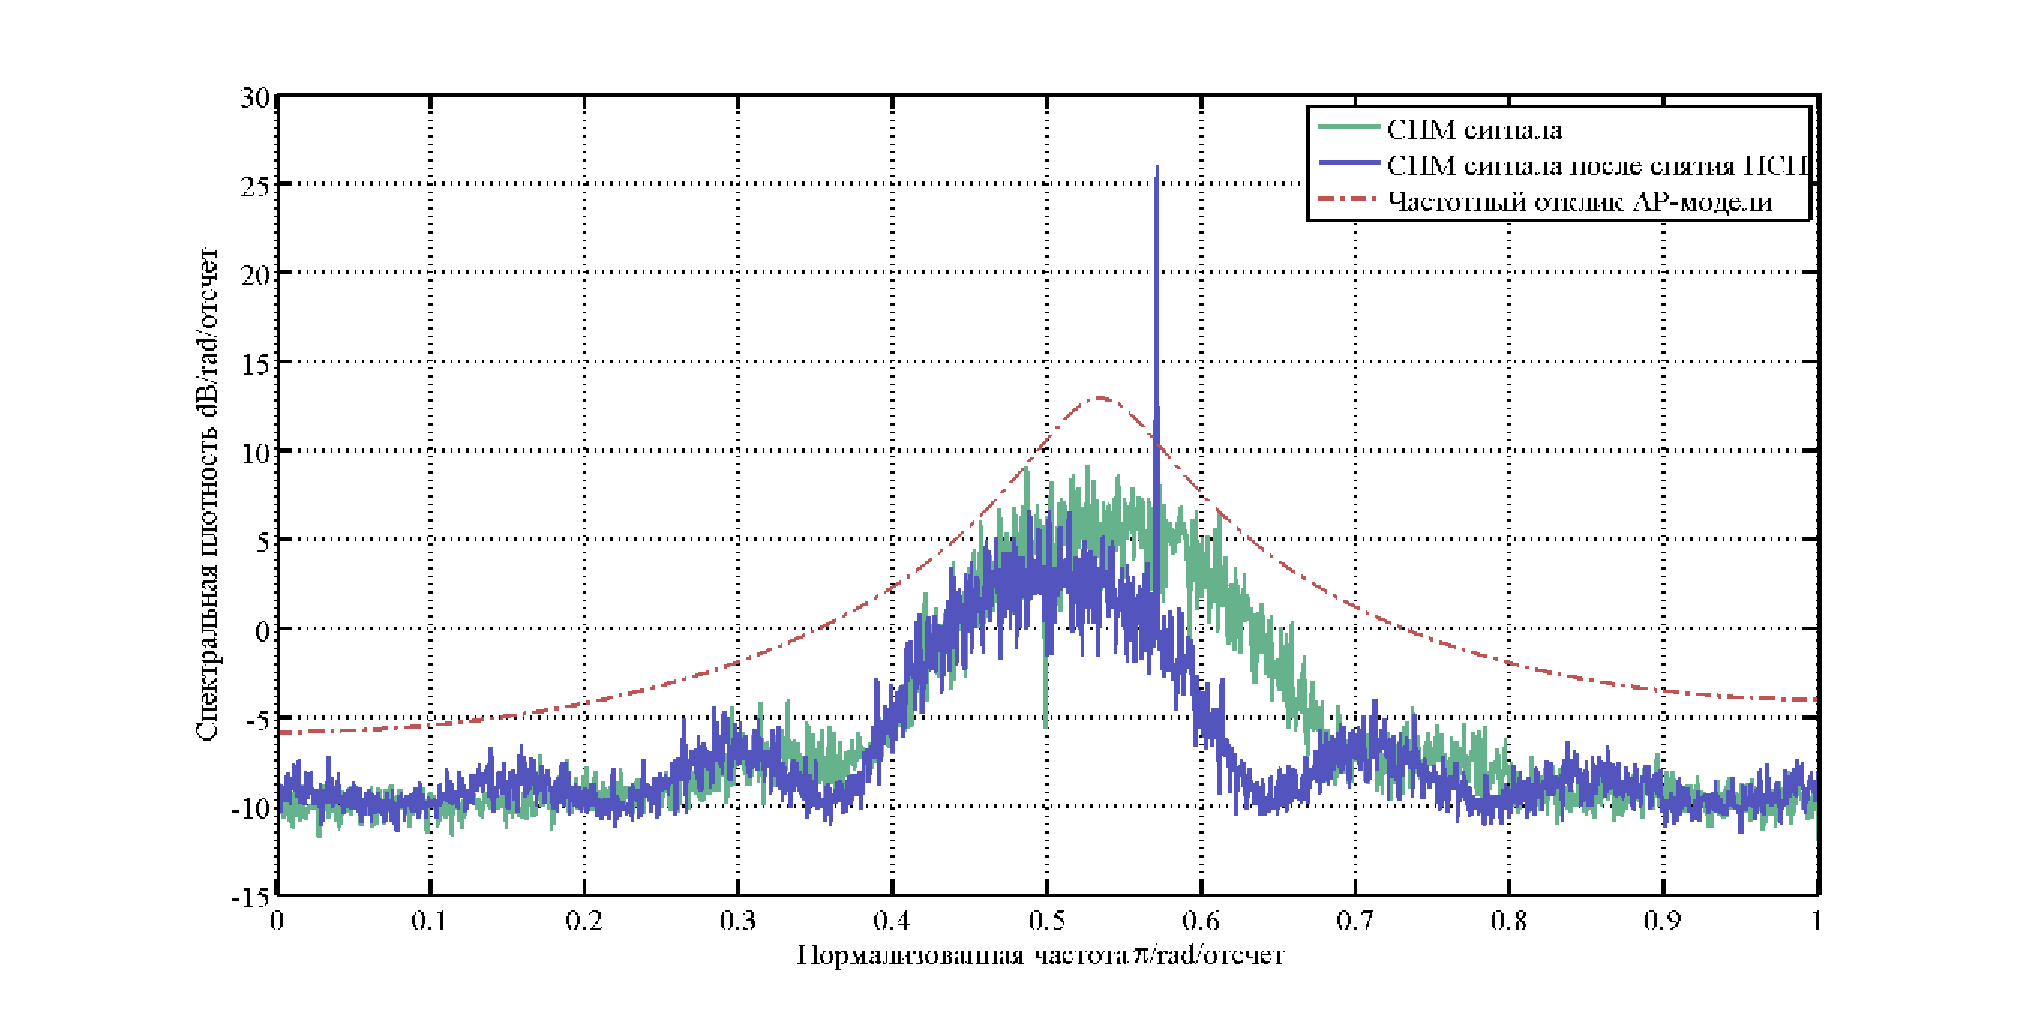
\includegraphics[width=1\linewidth]{lpc_2sat_psd.eps}}
	\caption{Оценка сигнала модулированного ПСП при наличии интерференции}
	\label{pic:ar_cdma1_freq_est2}
\end{figure}
